\def\epbold{\mbox{\boldmath$\epsilon$}}
\chapter{Basic Theory of Radiation Fields}
\label{cha:basic-theory-radi}

\section{Maxwell's Equations}
\label{sec:maxwells-equations}
\index{electrodynamics!Maxwell's equations}
Most of this material is probably familar, so this will only present a
quick review.  The goals are to understand how charges move under the
influence of electromagnetic fields, how when the charges accelerate,
they emit electromagnetic radiation and how this radiation transports energy.
The electric and magnetic field may be
defined operationally by observing the motion of a particle of charge
$q$ travelling through the field.  The force on the particle is given
by the Lorentz force equation,
\begin{equation}
{\bf F} = q \left ( {\bf E} + \frac{\bf v}{c} \times {\bf B} \right ).
\label{eq:124}
\end{equation}
The fields perform work on the particle at a rate
\begin{equation}
{\bf v}\cdot {\bf F} = q {\bf v} \cdot {\bf E}.
\label{eq:125}
\end{equation}
One can imagine an ensemble of charged particles of charge density
$\rho$ and define the current to be ${\bf J}=\rho {\bf v}$.  In this
case we find that power delivered on the charges per unit volume is
simply
\begin{equation}
P = {\bf J} \cdot {\bf E}.
\label{eq:126}
\end{equation}
Note that the magnetic field ${\bf B}$ does not perform work on the
particle.   It changes the direction of the particle's motion but not
its speed.

The equations that describe the dynamics of the fields are Maxwell's
equations,
\begin{eqnarray}
{\bf \nabla} \cdot {\bf D} = 4\pi \rho & {\bf \nabla} \cdot {\bf B} =
0 \nonumber \\
{\bf \nabla} \times {\bf H} = \frac{4\pi}{c} {\bf J} +\frac{1}{c} 
\pp{\bf D}{t}
& {\bf \nabla} \times {\bf E} = -\frac{1}{c} \pp{\bf B}{t} 
\label{eq:127}
\end{eqnarray}
in Gaussian units.   The fields ${\bf D}$ and ${\bf H}$ are related to
${\bf E}$ and ${\bf B}$ through the constitutive relations
\begin{equation}
{\bf D} = \epsilon {\bf E}, {\bf B} = \mu {\bf H}, 
\label{eq:128}
\end{equation}
where $\epsilon$ and $\mu$ are in general matrices that depend on the
fields applied, but in most situations they are constant scalars and
for a vacuum they are simply one.

The equations were discovered by various people.  Proceeding left to
right then top to bottom we have Gauss's law, a law without a name,
Ampere's law and Faraday's law.  It might be more appropriate to call 
the penultimate, Maxwell's equation, because Ampere's law as it was
originally formulated was
\begin{equation}
{\bf \nabla} \times {\bf H} = \frac{4\pi}{c} {\bf J} 
\label{eq:129}
\end{equation}
Maxwell added the term proportional to the rate of change of the
electric field.  If one takes the divergence of the complete Ampere's
law one obtains,
\begin{equation}
{\bf \nabla} \cdot \left ( {\bf \nabla} \times {\bf H} \right ) = 
\frac{4\pi}{c} {\bf \nabla} \cdot {\bf J}  +
\frac{1}{c} {\bf \nabla} \cdot \pp{\bf D}{t}
\label{eq:130}
\end{equation}
The left-hand side vanishes because the divergence of the curl
vanishes, on the right hand side one obtains,
\begin{equation}
0 = \frac{4\pi}{c} {\bf \nabla} \cdot {\bf J}  +
\frac{4\pi}{c} \pp{\rho}{t}
\label{eq:131}
\end{equation}
where we have used the first of Maxwell's equations to simply the
result and find that the Maxwell's addition makes the full set of
equations consistent with charge conservation.

Let's calculate the work that the field will do on a bunch of charges
per unit volume,
\begin{equation}
{\bf J} \cdot {\bf E} = \frac{1}{4\pi} \left [ c \left ({\bf \nabla}
  \times {\bf H} \right ) \cdot {\bf E} - {\bf E} \cdot 
\pp{\bf D}{t} \right ]
\label{eq:132}
\end{equation}
We have the following vector identity (the triple product)
\begin{equation}
{\bf E} \cdot  \left ({\bf \nabla}
  \times {\bf H} \right ) = 
{\bf H} \cdot  \left ({\bf \nabla}
  \times {\bf E} \right ) - 
{\bf \nabla}  \cdot  \left ({\bf E}
  \times {\bf H} \right ) 
\label{eq:133}
\end{equation}
Substituting in the earlier result and using Faraday's law yields,
\begin{equation}
{\bf J} \cdot {\bf E} = \frac{1}{4\pi} \left [ - {\bf H} \cdot
  \pp{\bf B}{t} 
- {\bf E} \cdot 
\pp{\bf D}{t} 
- c
{\bf \nabla}  \cdot  \left ({\bf E}
  \times {\bf H} \right ) 
 \right ]
\label{eq:134}
\end{equation}
Let's assume that $\epsilon$ and $\mu$ are constant and get
\begin{equation}
{\bf J} \cdot {\bf E} + \frac{1}{8\pi} 
\pp{}{t} 
\left [ {\bf H} \cdot {\bf B}
+  {\bf E} \cdot  {\bf D} \right ] + {\bf \nabla}  \cdot  \left ( \frac{c}{4\pi}
{\bf E}  \times {\bf H} \right ) = 0
\label{eq:135}
\end{equation}
This is Poynting's theorem.  We can identify the work performed on the
charges, the change in the field energy per unit volume and the flux
of field energy (${\bf S}$) as follows,
\begin{equation}
U_{ \hbox{\rm \scriptsize field}} = \frac{1}{8\pi} \left [ {\bf H} \cdot {\bf B}
+  {\bf E} \cdot  {\bf D} \right ] ~~\hbox{\rm and}~~ {\bf S} = \frac{c}{4\pi} {\bf E}
  \times {\bf H}
\label{eq:136}
\end{equation}
\index{electrodynamics!Poynting vector}

\subsection{Waves}
\label{sec:waves}
\index{electrodynamics!waves}
Let's look at Maxwell's equations in a vacuum,
\begin{eqnarray}
{\bf \nabla} \cdot {\bf E} = 0 & & {\bf \nabla} \cdot {\bf B} =
0 \nonumber \\
{\bf \nabla} \times {\bf E} = -\frac{1}{c} \pp{\bf B}{t} & &
{\bf \nabla} \times {\bf B} = +\frac{1}{c} 
\pp{\bf E}{t} 
\label{eq:137}
\end{eqnarray}
Let's take the curl of the third equation and combine it with the
fourth to get
\begin{equation}
{\bf \nabla} \times \left ({\bf \nabla} \times {\bf E} \right ) =
-\frac{1}{c^2} \pp{^2 {\bf E}}{t^2}
\label{eq:138}
\end{equation}
We have the identity that
\begin{equation}
{\bf \nabla} \times \left ({\bf \nabla} \times {\bf E} \right ) =
{\bf \nabla} \left ( {\bf \nabla} \cdot {\bf E} \right ) - {\bf
  \nabla}^2 {\bf E}.
\label{eq:139}
\end{equation}
The first term on the right-hand side vanishes so we get the final
wave equation,
\begin{equation}
 {\bf   \nabla}^2 {\bf E}
-\frac{1}{c^2} \pp{^2 {\bf E}}{t^2} = 0
\label{eq:140}
\end{equation}
and a similar equation for the magnetic field.

We write a general solution to the wave equation as a sum of
harmonically varying waves such as 
\begin{equation}
{\bf E}= \Re \left ({\bf \hat a}_1 E_0 e^{i({\bf k \cdot r}-\omega t)}
\right )
~~\hbox{\rm and}~~~
{\bf B}= \Re \left ( {\bf \hat a}_2 B_0 e^{i({\bf k \cdot r}-\omega
  t)} \right )
\label{eq:141}
\end{equation}
Application of Maxwell's equations to the above solutions shows 
\begin{equation}
\nabla \cdot {\bf E} = i {\bf k} \cdot {\bf E} =0 ~\rmmat{so}~
{\bf \hat a}_{1} \perp {\bf k}
\label{eq:142}
\end{equation}
\begin{equation}
\nabla \cdot {\bf B} = i {\bf k} \cdot {\bf B} = 0~\rmmat{so}~
{\bf \hat a}_{2} \perp {\bf k}
\label{eq:143}
\end{equation}
\begin{equation}
\nabla \times {\bf E} + \frac{1}{c} \pp{\bf B}{t} = 
i {\bf k} \times {\bf E} - i \frac{\omega}{c} {\bf B} = 0
~\rmmat{so}~{\bf \hat a}_{1} \perp {\bf \hat a}_{2}
\label{eq:144}
\end{equation}
\begin{equation}
\nabla \times {\bf B} - \frac{1}{c} \pp{\bf E}{t} = 
i {\bf k} \times {\bf B} + i \frac{\omega}{c} {\bf E} = 0
~\rmmat{so}~\omega=kc~\rmmat{and}~E_0=B_0.
\label{eq:145}
\end{equation}

We would like to calculate the time-averaged energy density and energy
flux assoicated with the wave.  In general $E_0$ and $B_0$ are complex
quantities.  First let's look at the Poynting vector
\begin{eqnarray}
\left < {\bf S} \right > &=& \frac{1}{P} \int_0^P
\frac{c}{4\pi} {\bf E \times B} d t \\
&=& \frac{c{\bf \hat k}}{4\pi P} \int_0^P \!\!\!\!\!\!
d t
 \left ( \Re E_0 \cos \omega t 
- \Im E_0 \sin \omega t \right ) \times \nonumber \\ & & ~~~ \left ( \Re B_0 \cos \omega t 
- \Im B_0 \sin \omega t \right )   \\
&=&  \frac{c{\bf \hat k}}{4\pi P} \int_0^P \!\!\!\!\!\!
d t
 \left ( \Re E_0 \Re B_0 \cos^2 \omega t + \Im E_0 \Im B_0 \sin^2
 \omega t \right ) \\
&=&  \frac{c{\bf \hat k}}{8\pi} 
 \left ( \Re E_0 \Re B_0 + \Im E_0 \Im B_0 \right ) =
\frac{c{\bf \hat k}}{8\pi} \Re E_0^* B_0 \\
&=& \frac{c{\bf \hat k}}{8\pi} |E_0|^2= \frac{c{\bf \hat k}}{8\pi} |B_0|^2
\label{eq:146}
\end{eqnarray}
The time-averaged energy density is
\begin{equation}
\left < U \right > = \frac{1}{16\pi} \Re \left ( E_0 E_0^* + B_0 B_0^*
\right ) = \frac{1}{8\pi} |E_0|^2 = \frac{1}{8\pi} |B_0|^2
\label{eq:147}
\end{equation}
Because the electric and magnetic field have the same behaviour we
only have to describe one of the fields to determine the properties of the
wave.  It is customary to focus on the electric field.

\subsection{The Spectrum}
\label{sec:spectrum}
\index{electrodynamics!spectrum} A general electromagnetic wave can be
expressed as a sum of the Fourier components described in the previous
section.  We have been characterizing the energy in the radiation
field with the quantity $I_\nu$ the intensity per unit frequency
interval.  It would be nice to find an relationship between the
electric field as a function of time and the intensity.

\index{Fourier transform}
The first step in obtaining the spectrum is to take a Fourier
transform of the electric field of the wave
\begin{equation}
{\hat E} (\omega) = \frac{1}{2\pi} \int_{-\infty}^{\infty} E(t)
e^{i\omega t} d t.
\label{eq:148}
\end{equation}
The inverse of the this is
\begin{equation}
E (t) =  \int_{-\infty}^{\infty} {\hat E}(\omega)
e^{-i\omega t} d \omega.
\label{eq:149}
\end{equation}
Because $E(t)$ is real find that ${\hat E}(-\omega)={\hat
  E}^*(\omega)$ so we don't have to keep track of the negative
frequencies.

To study the energy carried by the wave we look at the Poynting vector
\begin{equation}
\frac{d W}{d t d A} = \frac{c}{4\pi} E^2(t)
\ee 
The total energy per unit area in the wave is 
\begin{equation}
\frac{d W}{d A} = \frac{c}{4\pi} \int_{-\infty}^{\infty} E^2(t) dt
\label{eq:150}
\end{equation}
Parseval's theorem (see \S~\ref{sec:an-math-asid} for a proof) for Fourier transforms states that
\begin{equation}
\int_{-\infty}^{\infty} |E|^2(t) dt = 2\pi \int_{-\infty}^{\infty} 
|{\hat E}(\omega)|^2 d \omega.
\label{eq:151}
\end{equation}
Additionally, because ${\hat E}(-\omega)={\hat
  E}^*(\omega)$ we have
\begin{equation}
\int_{-\infty}^{\infty} E^2(t) dt = 4\pi \int_0^{\infty} 
|{\hat E}(\omega)|^2 d \omega.
\label{eq:152}
\end{equation}
and we can write
\begin{equation}
\frac{d W}{d A} = c \int_0^{\infty} 
|{\hat E}(\omega)|^2 d \omega.
\label{eq:153}
\end{equation}
And we obtain that 
\begin{equation}
\frac{d W}{d A d \omega } = c |{\hat E}(\omega)|^2
\label{eq:154}
\end{equation}
The intensity is related to the energy per unit time.   If the pulse
repeats on a time scale $T$ or the wave changes only on timescales $T$
much longer than $1/\omega$ we may define
\begin{equation}
\frac{d W}{d A d \omega d t} = \frac{c}{T} |{\hat E}(\omega)|^2
\label{eq:155}
\end{equation}
Table~\ref{tab:fourier} gives a few Fourier transforms of common
functions.  Although the last one seems rather arcane it has an important
property,
\begin{equation}
\int \frac{\sin \left [T    (\omega-\omega') \right ]}{\pi (\omega -
  \omega')} d\omega = 1
\label{eq:156}
\end{equation}
that lets us define the pair
\begin{eqnarray}
E(t) &=& e^{-i\omega' t} \\
{\hat E}(\omega) &=& \delta (\omega-\omega')
\label{eq:157}
\end{eqnarray}
where 
\begin{equation}
\int \delta(\omega-\omega') f(\omega) d\omega = f(\omega')
\label{eq:158}
\end{equation}

\begin{table}
\caption{Some Useful Fourier transforms}
\label{tab:fourier}
\begin{center}
\begin{tabular}{cc}
\hline \\
$E(t)$ &  ${\hat E}(\omega)$ \\  \\ \hline \\
\begin{minipage}[c]{0.3\columnwidth}
\begin{center}
\tikz \draw (0,0)--(0.5,0)--(0.5,0.5)--(1,0.5)--(1,0)--(1.5,0)
(0.75,0) node {$w$} (1.25,0.25) node {$h$}  (0.75,0.7) node {$t_0$};
\end{center}
\end{minipage}
& $\frac{h}{\pi \omega} \sin \frac{\omega w}{2} e^{i\omega t_0}$
 \\
\begin{minipage}[c]{0.3\columnwidth}
\begin{center}
\tikz \draw (0,0)--(0.5,0)--(0.75,0.5)--(1,0)--(1.5,0);
\end{center}
\end{minipage}
  & 
$\frac{2 h}{\pi w \omega^2} \left ( 1 - \cos \frac{\omega w}{2} \right ) e^{i\omega t_0}$
\\ \\
$\exp \left ( -\frac{\left(t-t_0\right)^2}{2\sigma^2} \right )$ & 
$e^{i\omega t_0} \exp
\left ( -\frac{\omega^2 \sigma^2}{2} \right )
\sqrt{\frac{\sigma^2}{2\pi}}$ \\ \\
$e^{-a|t|}$ &  $\frac{1}{2\pi} \frac{a}{a^2+\omega^2}$ \\ \\
$\exp \left ( - i \omega' t \right ) ~\hbox{\rm for}~ |t|<T$ &
$\frac{\sin \left [T    (\omega-\omega') \right ]}{\pi (\omega -
  \omega')}$ 
\\ \\
\hline
\end{tabular}
\end{center}
\end{table}

\section{Polarization}
\label{sec:polar-stok-param}
\index{electrodynamics!polarization}
\index{radiation!polarization}
For a general electromagnetic wave with wavenumber ${\bf k}$ we can
define a basis for the polarization of the wave:
$\epbold_1$ and $\epbold_2$ such that 
$\epbold_1 \times \epbold_2 ~\|~ {\bf k}$.   For example a wave can 
be linearly polarized with its electric field always pointing along 
$\epbold_1$ or along $\epbold_2$.   A
general solution is a linear combination of these two waves with
complex coefficients.  To be more specific we have
\begin{eqnarray*}
{\bf E}_1 &=& \epbold_1 E_1 e^{i{\bf k}\cdot {\bf x} - i \omega t} \\
{\bf E}_2 &=& \epbold_2 E_2 e^{i{\bf k}\cdot {\bf x} - i \omega t}\\
{\bf B}_j &=& \frac{{\bf k}\times {\bf E}_j}{k} \\
\label{sec:polar-stok-param-1}\end{eqnarray*}
and a general wave would be ${\bf E}={\bf E}_1 + {\bf E}_2$.  Because
the coefficients $E_1$ and $E_2$ are complex we can introduce a phase
difference between the two perpendicular components.  If this phase
difference is zero, then the wave is linearly polarized (left panel of
Fig.~\ref{fig:polar}) with the
polarization vector making an angle $\theta=\tan^{-1}(E_2/E_1)$ with
$\epbold_1$ and a magnitude of $E=\sqrt{E_1^2+E_2^2}$

\begin{figure}
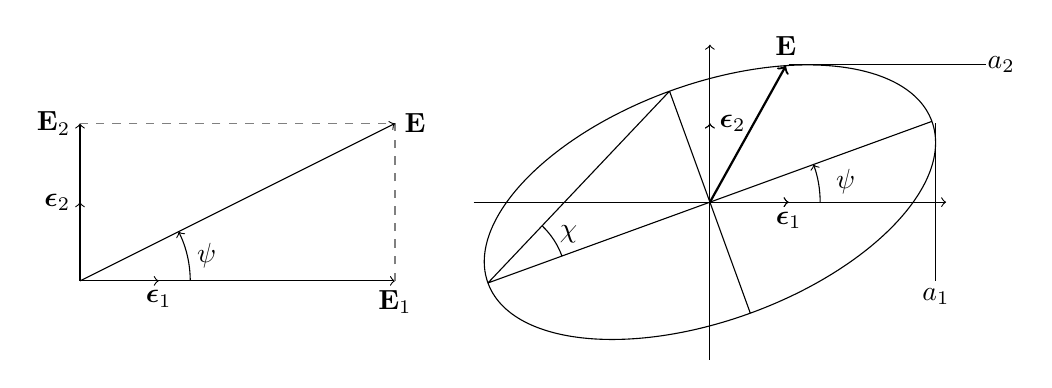
\begin{tikzpicture}
\draw [->] (0,0) -- (0,1) ;
\draw [->] (0,0) -- (0,2) ;
\draw [->] (0,0) -- (1,0) ;
\draw [->] (0,0) -- (4,0) ;
\draw [dashed,gray] (4,0) -- (4,2) -- (0,2) ;
\draw [->] (0,0) -- (4,2) ;
\draw [->] (1.4,0) arc (0:26.57:1.4) ;
\draw (1,0) node [below] {$\epbold_1$}  
(0,1) node [left]  {$\epbold_2$}
(4,0) node [below] {${\bf E}_1$}  
(0,2) node [left] {${\bf E}_2$}  
(4,2) node [right] {${\bf E}$} 
(13.28:1.4) node [right] {$\psi$} ;
\begin{scope}[shift={(8,1)}]
\draw (1,1.75)-- ++(2.5,0) ++(0.2,0) node {$a_2$}
(2.87,1)-- ++(0,-2) ++(0,-0.2) node {$a_1$};
\draw [rotate=20] (0,0) ellipse (3 and 1.5) (-3,0) -- (3,0) 
(0,-1.5) -- (0,1.5) 
(1.5,1.2990381057) node [above] {${\bf E}$} 
(-3,0) -- (0,1.5) (-2,0) arc (0:26.565834671:1) (-3,0)
++(18:1) node [right] {$\chi$};
\draw [->] (1.4,0) arc (0:20:1.4);
\draw [->] (0,0) -- (0,1) ;
\draw [->] (0,0) -- (1,0) ;
\draw [->] (0,0) -- (0,1) ;
\draw [->] (0,-2) -- (0,2) ;
\draw [->] (0,0) -- (1,0) ;
\draw [->] (-3,0) -- (3,0) ;
\draw [->,rotate=20,thick] (0,0) -- (1.5,1.2990381057);
\draw (1,0) node [below] {$\epbold_1$}  
(0,1) node [right] {$\epbold_2$}
(10:1.5) node [right] {$\psi$} ;
\end{scope}
\end{tikzpicture}
\caption{Electric field of linearly (left) and elliptically (right)
  polarized waves}
\label{fig:polar}
\end{figure}


If the phase difference is nonzero, one in genral has an elliptically
polarized wave as shown in the right panel of Fig.~\ref{fig:polar}.
The orientation of the ellipse is characterized by the
orientation, tile or azimuth angle $\psi$ which is the angle between
the semimajor axis of the ellipse and $\epbold_1$.  The shape of the
ellipse is measured by the ellipticity, $\epsilon$, the ratio of the
lengths of the major to minor axes.  We can also define an ellipticity
angle $\chi=\cot^{-1} \epsilon$.  The sign of $\chi$ is positive for
a right-hand circularly polarized wave --- in this case the electric field would
proceed anti-clockwise in Fig.~\ref{fig:polar}.

One could have defined an alternative representation based on the
circular polarizations
\begin{equation}
\epbold_\pm = \frac{1}{\sqrt{2}} \left ( \epbold_1 \pm i \epbold_2
\right ).
\label{eq:162}
\end{equation}
Because $\epbold_\pm$ is now complex one has to be a bit careful
about its orthogonality properties.  Specifically,
\begin{equation}
\epbold_\pm^* \cdot \epbold_\mp = 0,
\epbold_\pm^* \cdot {\bf k} = 0,
\epbold_\pm^* \cdot \epbold_\pm = 1.
\label{eq:163}\end{equation}
Often it is convenient to use this circular polarization basis rather
than the linear polarization basis above (for example, waves
travelling through plasma).

Most astronomical detectors blueward of the microwave measure not the
electric field directly but rather the energy delivered by the wave.
It is possible to recover this polarization information through
intensity measurements.

Generally one inserts a filter which collapses the incoming wave onto
one of the polarization states and one measures the resulting
intensity.  For example,  the intensity measured through a polarizing
filter aligned along the $1-$direction is $|\epbold_1 \cdot {\bf
  E}|^2$.   Let be more explicit and take two examples,
\begin{eqnarray*}
E_1 &=& a_1 e^{i\delta_1},~~~  E_2 = a_2 e^{i\delta_2} \\
E_+ &=& a_+ e^{i\delta_+},~~~  E_- = a_- e^{i\delta_-}.
\end{eqnarray*}
The first wave is given in the linear basis and the second is given in
the circular basis.  One typically makes a series of intensity
measurements through filters and quarter wave plates with different
orientations and combines the resulting intensities to form the
Stokes parameters, $I,Q,U$ and $V$ or $s_0,s_1,s_2$ and $s_3$.
The first parameter measures the total intensity of the wave, the sum
of the intensities of the two linearly polarized measurements.

\subsection{Stokes Parameters}
\index{radiation!Stokes parameters}
In the linear polarization basis we have
\begin{eqnarray*}
I &=& s_0 = |\epbold_1 \cdot {\bf E}|^2 + |\epbold_2 \cdot {\bf
  E}|^2 = a_1^2 + a_2^2 \\
Q &=& s_1 = |\epbold_1 \cdot {\bf E}|^2 - |\epbold_2 \cdot {\bf
  E}|^2 = a_1^2 - a_2^2 \\
U &=& s_2 = 2 \Re \left [ (\epbold_1 \cdot {\bf E})^* (\epbold_2 \cdot {\bf
  E}) \right ] = 2 a_1 a_2 \cos \left (\delta_2 - \delta_1 \right ) \\
V &=& s_3 = 2 \Im \left [ (\epbold_1 \cdot {\bf E})^* (\epbold_2 \cdot {\bf
  E}) \right ] = 2 a_1 a_2 \sin \left (\delta_2 - \delta_1 \right ) \\
\end{eqnarray*}
and for the circular basis we have 
\begin{eqnarray*}
I &=& s_0 = |\epbold_+ \cdot {\bf E}|^2 + |\epbold_- \cdot {\bf
  E}|^2 = a_+^2 + a_-^2 \\
Q &=& s_1 = 2 \Re \left [ (\epbold_+ \cdot {\bf E})^* (\epbold_- \cdot {\bf
  E}) \right ] = 2 a_+ a_- \cos \left (\delta_- - \delta_+ \right ) \\
U &=& s_2 = 2 \Im \left [ (\epbold_+ \cdot {\bf E})^* (\epbold_- \cdot {\bf
  E}) \right ] = 2 a_+ a_- \sin \left (\delta_- - \delta_+ \right ) \\
V &=& s_3 = |\epbold_+ \cdot {\bf E}|^2 - |\epbold_- \cdot {\bf
  E}|^2 = a_+^2 - a_-^2 \\
\end{eqnarray*}
The fractional polarization is given by
\begin{equation}
\Pi = \frac{\sqrt{Q^2+U^2+V^2}}{I}.
\label{eq:164}
\end{equation}
and the fractional linear polarization
\begin{equation}
\Pi_l = \frac{\sqrt{Q^2+U^2}}{I}.
\label{eq:165}
\end{equation}
The four Stokes parameters satisfy the following relationship for a
truly monochromatic wave
\begin{equation}
s_0^2 = s_1^2 + s_2^2 + s_3^2.
\label{eq:166}
\end{equation}

\subsection{Poincar\'e Sphere}
\index{radiation!Poincar\'e sphere}

This result shows that the Stoke's parameters live on a sphere of
radius $r\leq s_0$ where the extent of polarization $\Pi=r/s_0$.
This sphere of polarization is known as the Poincar\'e sphere
(Fig.~\ref{fig:poincare}) and the
location of the polarization on the sphere is related to the
orientation of the polarization ellipse in Fig.~\ref{fig:polar}.  In
particular we have
\begin{eqnarray*}
s_1 &=& Q = \Pi I \cos2\psi \cos 2\chi \\
s_2 &=& U = \Pi I \sin2\psi \cos 2\chi \\
s_3 &=& V = \Pi I \sin 2\chi
\end{eqnarray*}
which relates Stoke's parameters to the orientation and shape of the
polarization ellipse.  The two angles defined in Fig.~\ref{fig:polar}
related to the latitude ($2\chi$) and longitude ($2\psi$) of the
polarization vector $(s_1,s_2,s_3)$ on the Poincar\'e sphere.

\begin{figure}
\begin{center}
\input poincare
\end{center}
\caption{The Poincar\'e sphere}
\label{fig:poincare}
\end{figure}

An interesting and useful relationship is that the Stokes
parameters are additive for waves whose phases are not correlated.
Let's take two waves of frequencies $\omega_a$ and $\omega_b$ and
calculate the value of the first Stokes parameter as an example.  We have
\begin{eqnarray}
\label{eq:167}
I &=& s_0 = |\epbold_1 \cdot {\bf E}|^2 + |\epbold_2 \cdot {\bf
  E}|^2 \\
&=& \frac{1}{\Delta t} \int_0^{\Delta t}   \biggr [
\left |
\epbold_1 \cdot {\bf E}_a e^{-i\omega_a t} + \epbold_1 \cdot {\bf E}_b 
e^{-i\omega_b t} \right |^2 + \nonumber \\
& & ~~~~~~
\left |
\epbold_2 \cdot {\bf E}_a e^{-i\omega_a t} + \epbold_2 \cdot {\bf E}_b 
e^{-i\omega_b t} \right |^2 \biggr ] d t \\
&=& 
\frac{1}{\Delta t} \int_0^{\Delta t}   \biggr \{
\left | \epbold_1 \cdot {\bf E}_a \right |^2  +
\left |  \epbold_1 \cdot {\bf E}_b \right |^2 +
\left | \epbold_1 \cdot {\bf E}_a \right |^2  +
\left |  \epbold_1 \cdot {\bf E}_b \right |^2 + \nonumber \\
& & ~~~ 
2 \left [ \left ( \epbold_1 \cdot {\bf E}_a \right ) 
\left ( \epbold_1 \cdot {\bf E}_b \right ) +
\left ( \epbold_2 \cdot {\bf E}_a \right ) 
\left ( \epbold_2 \cdot {\bf E}_b \right )  \right ]
\cos \left [ \left (\omega_a-\omega_b\right ) t \right ] \biggr \}
\label{eq:168} \\
&=& s_{0,a} + s_{0,b} + 
\left \{ 
\begin{array}{cl}
\mathcal{O} \left [ \sqrt{s_{0,a}
      s_{0,b}}
 \left ( \Delta \omega \Delta t \right)^{-1} \right ]
& \Delta\omega \Delta t \gg 1 \\
\mathcal{O} \left [ \sqrt{s_{0,a}
      s_{0,b}} \left ( \Delta \omega \Delta t \right )  \right ]
& \Delta\omega \Delta t \ll 1 
\end{array} \right .
\end{eqnarray}
where $\Delta \omega = \omega_a-\omega_b$. For example, if we look at
a star over a wide range of frequencies (the definition of wide is 
$\Delta \omega \Delta t \gg\ 1$), the phase of waves at one end of the 
frequency range will not correlate with waves at the other end.  

When we measure the Stokes parameters in practice we measure for example
\begin{equation}
s_2 = 2 \left < a_1 a_2 \cos \left (\delta_2 - \delta_1 \right )
\right >.
\label{eq:169}
\end{equation}
Although $\cos^2 x + \sin^2 x = 1$, $0\leq \left <\cos x\right>^2  +
\left <\sin x\right>^2 \leq 1$, so for a quasimonochromatic wave we
have
\begin{equation}
s_0^2 \geq s_1^2 + s_2^2 + s_3^2.
\label{eq:170}
\end{equation}
Because the Stokes parameters are additive and measure the energy
content of the wave, they are a natural basis to calculate the
radiative transfer of polarized radiation.

\section{Electromagnetic Potentials}
\label{sec:electr-potent}
\index{electrodynamics!potentials}
Looking at the structure of Maxwell's equations, we can see that we can 
express the magnetic field as the curl of another field, the vector potential,
\begin{equation}
\nabla \cdot {\bf B} = \nabla \cdot (\nabla \times {\bf A}) = 0 
\label{eq:171}
\end{equation}
where the second equality is an identity if ${\bf B} = \nabla \times
{\bf A}$. 

Let's substitute this into the other homogenous Maxwell
equation,
\begin{eqnarray}
\nabla \times {\bf E} + \frac{1}{c} \pp{}{t} \nabla \times {\bf A} &=& 0 \\*
\nabla \times \left ( {\bf E} + \frac{1}{c} \pp{\bf A}{t} \right ) &=& 0
\end {eqnarray}
If
\begin{equation}
-\nabla\phi =  {\bf E} + \frac{1}{c} \pp{\bf A}{t} 
\label{eq:172}
\end{equation}
then the second homogeneous Maxwell equation is satisfied as well.

Let's recap
\begin{eqnarray}
{\bf B} &=& \nabla \times {\bf A} \\
{\bf E} &=& -\nabla \phi - \frac{1}{c} \pp{\bf A}{t} \\
\label{eq:173}
\end{eqnarray}
The expression of the fields in terms of the vector and scalar
potential guarantees that two out of four of Maxwell's equations are
satisfied.  Let's substitute our results into the remaining Maxwell's
equations,
\begin{eqnarray}
\nabla \cdot {\bf E} &=& 4\pi\rho \\
\nabla \cdot \left ( -\nabla \phi - \frac{1}{c} \pp{\bf A}{t} \right ) &=& 4\pi \rho \\
\nabla^2 \phi +  \frac{1}{c} \pp{}{t} \nabla \cdot {\bf A}&=& -4\pi \rho
\label{eq:174}
\end{eqnarray}
and the second inhomogeneous equation gives
\begin{eqnarray}
\nabla \times {\bf B} - \frac{1}{c} \pp{\bf E}{t} &=& \frac{4\pi}{c} {\bf J} \\
\nabla \times \left ( \nabla \times {\bf A} \right ) + \frac{1}{c} \pp{}{t} \left ( \nabla \phi + \frac{1}{c} \pp{\bf A}{t} \right )&=& \frac{4\pi}{c} {\bf J} \\
\nabla \left ( \nabla \cdot {\bf A} \right ) - \nabla^2 {\bf A} + \frac{1}{c} \pp{}{t} \left ( \nabla \phi + \frac{1}{c} \pp{\bf A}{t} \right )&=& \frac{4\pi}{c} {\bf J} 
\label{eq:175}
\end{eqnarray}
Now let's rearrange the last equation a bit more,
\begin{eqnarray}
-\nabla \left ( \nabla \cdot {\bf A} \right ) +  \nabla^2 {\bf A} - \frac{1}{c} \pp{}{t} \left ( \nabla \phi \right ) - \frac{1}{c^2} \pp{^2 {\bf A}}{t^2} &=& -\frac{4\pi}{c} {\bf J}  \\
  \nabla^2 {\bf A}
- \frac{1}{c^2} \pp{^2 {\bf A}}{t^2}
-\nabla \left ( \nabla \cdot {\bf A}  + \frac{1}{c} \pp{\phi}{t}  \right ) &=& -\frac{4\pi}{c} {\bf J} 
\label{eq:176}
\end{eqnarray}
Let's look at the last of the charge density equations equations some more,
\begin{eqnarray}
\nabla^2 \phi +  \frac{1}{c} \pp{}{t} \nabla \cdot {\bf A}&=& -4\pi \rho \\*
\nabla^2 \phi - \frac{1}{c^2} \pp{^2 \phi}{t^2} +  \frac{1}{c} \pp{}{t} \left ( \nabla \cdot {\bf A}
+\frac{1}{c} \pp{\phi}{t} \right )&=& -4\pi \rho 
\label{eq:177}
\end{eqnarray}
Although it looks like that the equation is a bit more complicated than before, it now 
has the precise form of the equation with the current.   

Wouldn't life be simpler if the quantity in the parenthesis in both equations vanished?
Guess what?   We can choose for it to vanish by making a good choice
of gauge.  Only the electric and magnetic fields are measurable so we
can make any change to the potentials ${\bf A}$ and $\phi$ that we
want as long at ${\bf E}$ and ${\bf B}$ remain unchanged.  Because
${\bf B} = \nabla \times {\bf A}$ we can add the gradient of any
function $\psi$ to ${\bf A}$ without changing ${\bf B}$ (the curl of a
gradient of a function is zero).

However, if we add a gradient of function to ${\bf A}$ the value of
${\bf E}$ is affected,
\begin{equation}
{\bf E} \rightarrow {\bf E} - \frac{1}{c} \pp{}{t}
\nabla \psi.
\label{eq:178}
\end{equation}
To fix this we also have to change the scalar potential $\phi$ at the
same time by subtracting  $1/c ( \partial \psi/\partial t )$ from
$\phi$.   Therefore, we find that the equations of electromagnetism
remain unchanged if one replaces
\begin{equation}
{\bf A} \rightarrow {\bf A} + \nabla \psi ~~\hbox{\rm and}~~ \phi \rightarrow \phi -
\frac{1}{c} \pp{\psi}{t}
\label{eq:179}
\end{equation}
This is the gauge transformation and it means that we in general have
the freedom to set a particular scalar constraint on the potentials.

\subsection{Lorenz Gauge}
\index{electrodynamics!Lorenz gauge}

In particular we would like to set
\begin{equation}
 \nabla \cdot {\bf A}
+\frac{1}{c} \pp{\phi}{t} = 0
\label{eq:180}
\end{equation}
This is equivalent to finding a function $\psi$ that satisfies
\begin{equation}
\nabla^2 \psi - \frac{1}{c^2} \pp{^2 \psi}{t^2} +\nabla \cdot {\bf A}
+\frac{1}{c} \pp{\phi}{t} = 0
\label{eq:181}
\end{equation}
and adding it to ${\bf A}$ to get ${\bf A}'$.  It turns out that this
is possible so we are free to use the following equations for the
potentials,
\begin{equation}
\nabla^2 \phi - \frac{1}{c^2} \pp{^2 \phi}{t^2} =
-4\pi \rho,~~\hbox{\rm and}~~
  \nabla^2 {\bf A}
- \frac{1}{c^2} \pp{^2 {\bf A}}{t^2} =
-\frac{4\pi}{c} {\bf J}.
\label{eq:182}
\end{equation}
This is the Lorenz gauge (which happens to be {\em Lorentz}
invariant).

\subsection{Green's Function}

Both of the equations have the same form.  Let's look at the equation
for the electric field
\begin{equation}
\nabla^2 \phi - \frac{1}{c^2} \pp{^2 \phi}{t^2} = -4\pi \rho 
\label{eq:804}
\end{equation}
and write $\phi$ and $\rho$ in terms of their Fourier transforms in
time, e.g.
\begin{equation}
\rho({\bf r},t) = \int_{-\infty}^\infty \hat \rho ({\bf r}, \omega)
e^{-i\omega t} d t
\label{eq:805}\end{equation}
so the equation for the potential now looks like
\begin{equation}
\nabla^2 \hat \phi({\bf r},\omega) + \frac{\omega^2}{c^2} \hat \phi({\bf
  r},\omega) = -4\pi \hat \rho(\bf r,\omega) .
\label{eq:806}\end{equation}
Now let's look for a particular solution $G({\bf r},\omega)$ for $\hat
\phi$ where $\hat \rho$ vanishes everywhere but the origin
\begin{equation}
\nabla^2 \hat G({\bf r},\omega) + \frac{\omega^2}{c^2} \hat G({\bf
  r},\omega) = -4\pi \delta(\bf r).
\label{eq:807}\end{equation}
The function $G({\bf r},\omega)$ is the Green's function of the
equation (Eq.~\ref{eq:806}).   It is a useful concept because
Maxwell's equations are linear, so the principle of superposition
applies.  The electromagnetic fields for two charges is simply the sum
of the fields of each charge on its own.

Because the right-hand side only depends on the magnitude
of ${\bf r}$, the Green's function must be spherically symmetric, so
\begin{equation}
\frac{1}{r} \pp{^2}{r^2} \left [ r \hat G(r,\omega) \right ] + \frac{\omega^2}{c^2} \hat G(r,\omega) = -4\pi \delta(r)
\label{eq:808}
\end{equation}
which is nearly the equation for the potential for a point change.

We can start with the solution $1/r$ and add an exponential term to
handle the second term in the equation; let's substitute the following
ansatz
\begin{equation}
\hat G(r,\omega) = \frac{e^{ikr}}{r}
\label{eq:809}
\end{equation}
which yields
\begin{equation}
-k^2 \frac{e^{ikr}}{r} + \frac{\omega^2}{c^2} \frac{e^{ikr}}{r} =
-4\pi \delta(r)
\label{eq:812}
\end{equation}
which trivially solves the equation everywhere but the origin if 
$k=\pm \omega/c$.  Because Eq.~\ref{eq:808} is a second-order
differential equation we get two solutions,
\begin{equation}
{\hat G}^{\pm}(r,\omega) = \frac{e^{i \pm r \omega/c}}{r}
\label{eq:810}
\end{equation}
and the complete solution is a linear combination of the two.  Now
because we know the solution for source at a point we can write the
solution for a distribution of charge
\begin{equation}
\hat \phi^{\pm}({\bf r}, \omega) = \int d^3 r' \frac{\exp \left (
    \pm i\omega/c |{\bf r}-{\bf r}'|/c \right )  }{|{\bf r}-{\bf r}'|} \hat \rho({\bf r}',\omega) 
\label{eq:811}
\end{equation}
and write out the potential as a function of time
\begin{equation}
\phi^{\pm}({\bf r}, t) = \int d^3 r' d \omega \frac{\exp \left [
    -i\omega \left ( t \mp |{\bf r}-{\bf r}'|/c \right ) \right
  ]}{|{\bf r}-{\bf r}'|} \hat \rho({\bf r}',\omega) .
\label{eq:813}
\end{equation}
We can perform the integral over time because it is the same as
Eq.~(\ref{eq:805}) but with $t$ replaced by $t \mp |{\bf r}-{\bf
  r}'|/c$, so we have
\begin{equation}
\phi^{\pm}({\bf r}, t) = \int d^3 r' \rho \left ({\bf r}, t \mp
\frac{|{\bf r}-{\bf r}'|}{c} \right ) \frac{1}{|{\bf r}-{\bf r}'|}.
\label{eq:824}
\end{equation}

The solution for the vector potential is similar.  We have two choices
(or a linear combination).  The potential here can depend on the
locations of charges along the past and the future light cones.
Although the latter choice appears to violate causality, it all
really depends on what questions that you would like to ask.  For
example, if you wanted to know given the distribution of fields here
and now, what would be the distribution of charges to absorbed the
radiation in the future, then the {\bf advanced} potential (with the plus
sign after the time coordinate).   Here we are generally interested in
the radiation that a configuration of charges emit, so we shall use
the {\bf retarded} potentials,
\begin{eqnarray}
{\bf A}({\bf r},t) &=& \frac{1}{c} \int d^3 r' \frac{{\bf J}\left ({\bf
  r}',t-\frac{|{\bf r}-{\bf r}'|}{c} \right )}{|{\bf r} -
{\bf  r}'|} \\
\phi({\bf r},t) &=& \int d^3 r' \frac{\rho\left ({\bf
  r}',t-\frac{|{\bf r}-{\bf r}'|}{c} \right )}{|{\bf r} -
{\bf  r}'|} .
\label{eq:183}
\end{eqnarray}

\section{Further Reading}

To learn more about faint x-ray structure in the Crab nebula, consult
\begin{itemize}
\item Seward, F.~D., Tucker, W.~H. \& Fesen, R.~A.\ 2006, ``Faint X-Ray Structure in the Crab Pulsar Wind Nebula,'' {\em ApJ}, 652, 1277 
\end{itemize}
and 
\begin{itemize}
\item Heyl, J.~S. \& Shaviv, N.~J.\ 2000, ``Polarization evolution in
  strong magnetic fields,'' {\em MNRAS}, 311, 555 
\end{itemize}
use the Poincar\'e sphere extensively to study how the polarization of
emission from the surface of the Crab pulsar changes as it travels
through the star's magnetic field.

The general development of Maxwell's equations and the polarization of
radiation are examined in Chapter~6 and \S\S~7.1-7.2 of
\begin{itemize}
\item Jackson, J. D., {\em Classical Electrodynamics}.
\end{itemize}

\section{Problems}

\begin{enumerate}
\item{\bf  Coulomb's Law}

Derive Coulomb's law from Maxwell's Equations.

\item {\bf Ohm's Law and Absoption:} 

In certain cases the process of aborption of radiation can be treated
by means of the macroscopic Maxwell equations. For example, suppose we
have aconducting medium so that the current density ${\bf j}$ is related to
the electric field ${\bf E}$ by Ohm's law: ${\bf J} = \sigma {\bf E}$ where
$\sigma$ is the conductivity (cgs unit = $\mathrm{sec}^{-1}$). Investigate the
propagation of electromagnetic waves in such a medium and show that:
\begin{enumerate}
\item The wave vector ${\bf k}$ is complex
$$
{\bf k}^2 = \frac{\omega^2 m^2}{c^2}
$$
where $m$ is the complex index of refraction with
$$
m^2 = \mu \epsilon \left ( 1 + \frac{4 \pi i \sigma}{\omega \epsilon}
\right )
$$
\item The waves are attenuated as they propagate, corresponding to an
absorption coefficient.
$$
\alpha = \frac{2\omega}{c} \Im (m)
$$

\end{enumerate}

\begin{figure}
\begin{center}
\includegraphics[width=0.5\columnwidth]{crab_scale.jpg}
\end{center}
\caption{A Chandra image of the outskirts of the Crab pulsar wind
  nebula. Credit: NASA/CXC/SAO/F.Seward et al }
\label{fig:crab-edge}
\end{figure}

\item {\bf The Edge of the Crab}

  Fig.~\ref{fig:crab-edge} shows the x-ray emission of the Crab pulsar
  wind nebula at a distance of 2~kpc.  The x-ray emitting gas is
  contained by magnetic fields causing the x-ray emission regions to
  end sharply.  We can relate the frequency of the emission to the energy
  of the electrons and the strength of the magnetic field by
\begin{equation}
\omega = \left ( \frac{E}{m_e c^2}
\right )^2 \frac{e B}{m_e c} 
\end{equation}
and assume that the electrons are relativistic so their inertial mass
is $E/c^2$.  Use the sharpness of the emission
regions to determine the energy of the electrons and the strength of
the magnetic field.

\item {\bf Momentum and Angular Momentum: } 

This problem is meant to deduce the momentum and angular momentum
properties of radiation and does not recesarily represent any real
physical system of interest. Consider a charge $Q$ in a viscous medium
where the viscous force is proportional to velocity: 
$$
F_\rmscr{visc} = -\beta v
$$
Suppose a circular polarized wave passes through the medium. The
equation of motion of the charge is 
$$
m \dd{v}{t} = F_\rmscr{visc} + F_\rmscr{Lorentz}
$$
We assume that the terms on the right dominate the inertial term on the
left, so that approximately 
$$
0 = F_\rmscr{visc} + F_\rmscr{Lorentz}
$$
Let the frequency of the wave be $\omega$ and the strength of the
electric field be E.
\begin{enumerate}
\item
Show that to lowest order (neglecting the magnetic force) the crage
moves on a circle in a plane normal to the direction of propagation of
the wave with speed $QE/\beta$ and with radius $QE/(\beta \omega)$.
\item
Show that the power transmitted to the fliud by the wave is $Q^2 E^2/\beta$
\item
By considering the small magnetic force acting on the particle show
that the momentum per unit time (force) given to the fluid by the wave
is in the direction of propagation and has the magnitude 
$Q^2 E^2/(\beta c)$
\item
Show that the angular momentum per unit time (torque) given to the
fliud by the wave is in the direction of propagation and has magnitude
$\pm Q^2 E^2/(\beta \omega0$ where the + is for left and - is for
right circular polarization.
\item
Show that the absorption cross section of the charge is
$4\pi Q^2/(\beta c)$.
\item
 If we regard the radiation to be composed of circular polarized
 photons of energy $E_\gamma= h \nu$, show that these results imply that the
 photon has momemtum $p=h/\lambda=E_\gamma/c$ and has angular momemtum 
$J=\pm \hbar$ along the direction of propagation.
\item
 Repeat this problem for a linearly polarized wave
\end{enumerate}

\item {\bf Maxwell's equations before Maxwell: }

Show that Maxwell's equations before Maxwell, that is, without the
"displacement current" term, $c^{-1} \pp{D}{t}$, unacceptably constrained the
sources of the field and also did not permit the existence of waves.

\item {\bf Coulomb gauge} 
Derive the equations describing the dynamics of the electric and
vector potentials in the Coulomb gauge
$$
\nabla \cdot {\bf A} = 0
$$
Look at the equation for the electric potential. What is the solution
to the electric potential given the charge density $\rho$? Why is this
called the Coulomb gauge?

How does the expression for the scalar potential in the Coulomb gauge
differ from that in the Lorenz gauge? What is strange about it? Is it
physical?

Now look at the equation for the vector potential. Show that the LHS
can be arranged to be the same as in the Lorenz gauge but the RHS is
not just the current but the current plus something else.

Show that the RHS can be expressed as 
$$
\frac{4\pi}{c} \left ( {\bf J} - {\bf J}_\rmscr{long} \right ) 
$$
where
$$
{\bf J}_\rmscr{long} = -\frac{1}{4\pi} \nabla \int \frac{\nabla' \cdot
{\bf J}}{|{\bf x}-{\bf x}'|} d^3 x
$$
\end{enumerate}

%%% Local Variables:
%%% TeX-master: "book"
%%% End:
